\documentclass[12pt]{article}
\usepackage[a4paper, total={6in, 8in}]{geometry} % Margenes
\usepackage{amsmath} % Integrales, funciones a tramos, etc
\usepackage{graphicx} % Para incluir imagenes
\usepackage{subcaption} % Para crear subfiguras (ej. varias imagenes)
\graphicspath{{/home/franco/Facultad/AnalisisII/}}

\title{Resumen de temas del segundo parcial de Analisis Matemático II}

\begin{document}
\maketitle
\section{Definicion de integral doble sobre un rectángulo}
\par
La integral doble sobre un rectangulo $R$ con sus lados paralelos
a los ejec coordenados se puede aproximar dividiendo en $n\times m$ subrectangulos
al area con ancho $\Delta x$ y altura $\Delta y$ constantes. 
$$ R = (\Delta x \times n)( \Delta y \times m)$$
Para cada subrectangulo su area será $\Delta A = \Delta x \Delta y$ y la suma
de los productos entre area y la imagen de la función en un punto muestra
dentro del subrectangulo será una aproximación al valor de la integral en $R$.
$$\sum_i^n \sum_j^m f(x_i,y_j)\Delta A$$
Por lo tanto si $n, m \to \infty$, el límite de la doble suma de Riemann es igual
a la integral en $R$.
$$\lim_{n, m \to \infty}\sum_i^n \sum_j^m f(x_i,y_j)\Delta A = \iint_R f(x, y)\,dA$$

\section{Propiedades}
1. $$\iint_R [f(x,y) + g(x,y)]\,dA = \iint_R f(x,y)\,dA + \iint_R g(x,y) \,dA$$
\smallskip
2. $$\iint_R cf(x,y)\,dA = c \iint_R f(x,y)\,dA$$
\smallskip
3. Si $f(x,y) \geq g(x,y)$ para todo $ (x,y) \in R$, entonces
$$\iint_R f(x,y)\,dA \geq \iint_R g(x,y)\,dA$$

\section{Integrales Iteradas}
Son una forma de resolver integrales dobles con integrales parciales o de una
sola variable. Si $R = [a,b]\times[c,d]$ entonces 
$$\iint_R f(x,y)\,dA = \int_a^b[\int_c^d f(x,y)\,dy]\,dx$$
El método consiste en integrar primero a la funcion con respecto a una de las
variables, dejando constante a la otra para luego integrar la funcion resultante
con respecto a la otra variable. Se integra primero con respecto a la variable 
ubicada adentro, en este caso $y$.\\
\smallskip
\textbf{Teorema de Fubini:}  si la función es continua en $R$, 
la integral es igual independientemente del orden de integración:
$$\iint_R f(x,y)\,dA = \int_a^b[\int_c^d f(x,y)\,dy]\,dx = \int_c^d[\int_a^b f(x,y)\,dx]\,dy$$

\section{Integrales dobles sobre regiones generales}
Para calcular la integral de $f(x,y)$ sobre regiones diferentes de un rectangulo, primero se
define una funcion $$F(x,y) = \begin{cases} f(x,y) & (x,y) \in D\\0 & (x,y) \not \in D\end{cases}$$
con dominio en un rectangulo que contiene a la region original $D$. De manera que se pueda calcular
la integral $$\iint_R F(x,y)\,dA = \iint_D f(x,y)\,dA$$
La forma practica de resolver integrales dobles con esta idea es graficar la region de integracion
e identificar regiones de dos posibles tipos:\\
\begin{itemize}
\item \textbf{Tipo I} La region yace entre las graficas de dos funciones continuas de $x$
por lo que la integral para esa region sera $\int_a^b\int_{f(x)}^{g(x)} f(x,y) \,dy\,dx$
\item \textbf{Tipo II} La region yace entre las graficas de dos funciones continuas de $y$
por lo que la integral para esa region sera $\int_c^d\int_{f(y)}^{g(y)} f(x,y) \,dx\,dy$
\end{itemize}
\begin{figure}[h!]
    \centering
    \begin{subfigure}{0.4\linewidth}
        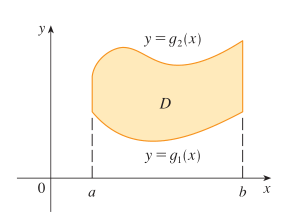
\includegraphics[width=\linewidth]{tipo1.png}
        \caption{Tipo 1.}
        \end{subfigure}
    \begin{subfigure}{0.4\linewidth}
        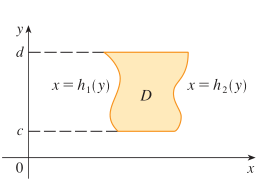
\includegraphics[width=\linewidth]{tipo2.png}
        \caption{Tipo 2.}
        \end{subfigure}
        \end{figure}
        
Si la region total sobre la que se quiere calcular la integral no puede ser definida como
una de ninguno de los dos tipos, debe ser dividida en subregiones que si pertenezcan a algun
tipo y luego sus resultados deben ser sumados.\\
Es posible dividir en subregiones a la region a integrar ya que una de las propiedades de las
integrales dobles es:
$$\iint_D f(x,y)\,dA = \iint_{D_1} f(x,y)\,dA + \iint_{D_2} f(x,y)\,dA$$
donde $D_1$ y $D_2$ son dos subregiones que no se superponen excepto en sus limites y conforman
la region total.
\section{Area de una region general}
Para calcular el area de una region plana se debe integrar a la funcion constante $f(x,y) = 1$
sobre la region plana. Entonces
$$\iint_D 1 \,dA = A(D)$$
\section{Integrales dobles en coordenadas polares}
Algunas regiones son mas faciles de expresar en coordenadas polares que en coordenadas
rectangulares, por ejemplo un circulo o un anillo. Para estos casos se puede cambiar 
una integral doble a polares para obtener el mismo resultado de manera mas sencilla.
Si $f$ es continua en un rectangulo polar $0\leq a \leq r \leq b, \alpha \leq \theta \leq \beta$:
$$\iint_R f(x,y)\,dA = \int_{\alpha}^{\beta}\int_a^b f(r cos\theta, r sin\theta) r \,dr \,d\theta$$
Este caso es el de rectangulos polares, pero tambien pueden evaluarse integrales para regiones mas
generales en coordenadas polares distinguiendo regiones y subregiones de dos tipos, de forma similar
al metodo para coordenadas rectangulares. En polares las regiones pueden encontrarse entre dos funciones
de la forma $\theta(r)$ o dos funciones $r(\theta)$. Luego una de las integrales iteradas tendra
extremos de integracion constantes y la otra tomara las expresiones de las funciones que encierren
a la region.
\section{Aplicaciones de integrales dobles}
\subsection{Densidad y masa}
\end{document}
